\section{Reimplementation Strategy}
\label{sec:remplementation}

The main purpose of my implementation work was to be able to code by myself some of the core ideas of the ADOP differentiable point based neural renderer.
I decided to code everything from scratch knowing since the start that I would at no point be able to fully reproduce the results from the authors but I learnt a large amount of things by doing so.
\begin{itemize}
    \item I used BlenderProc \cite{Denninger2023} to script and generate multiple synthetic scenes from the samples used in the NerF paper. All camera positions are known and share the same referential as my pytorch point renderer.
    \item A perfect point cloud is sampled at random from the mesh (through the .obj file).
    \item A pytorch function allows to project the points onto the image plane and includes soft depth test and normal culling.
\end{itemize}

Each element has been carefully tested by mostly visual tests.


Assumptions for simplification compared to the original ADOP paper. 
% TODO: FINISH
\begin{itemize}
    \item 
\end{itemize}



\subsection{Generating synthetic calibrated scenes}
\label{sec:synthetic_calibrated_scenes}
In order to avoid dealing with large real scenes with millions of points and having to deal with heavy COLMAP processing, I decided to use a recent library named BlenderProc  \cite{Denninger2023} which simplifies the use of Blender as it allows running renders in the background (launched through terminal without the need of a graphical user interface).

It is first possible to generate a set of viewpoints configurations to orbit around the scene. It is also possible to generate an environment map (e.g. a skybox). We render with the background transparency option so the rendering results is a RGB PNG. 
% 1532.9s for 60 views of the \texttt{material balls}.
% 753.869 ficus

% Rendering is peformed using GPU and requires 25 seconds per view with a resolution 640x480 for the \texttt{material balls}. scene on a laptop Nvidia T500.
% 27 minutes are needed to generate 64 viewpoints
\begin{figure}[H]
    \centering
    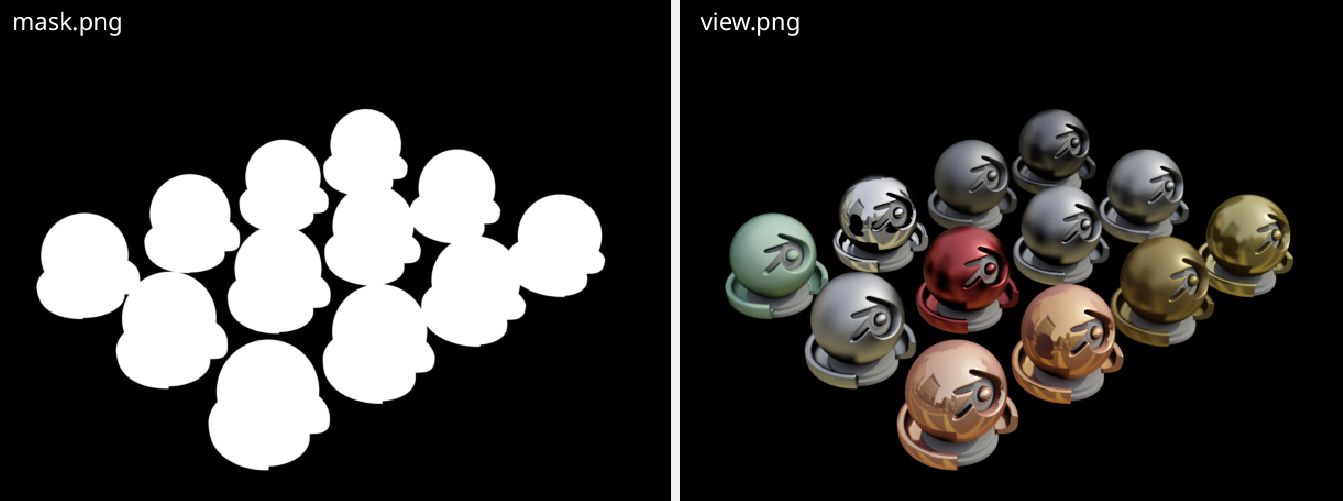
\includegraphics[width=0.5\textwidth]{figures/blenderproc_renders.png}
    \caption{Mask and RGB render BlenderProc renders with an environment map.}
    \label{fig:blenderproc_renders}
\end{figure}

\begin{figure}[H]
    \centering
    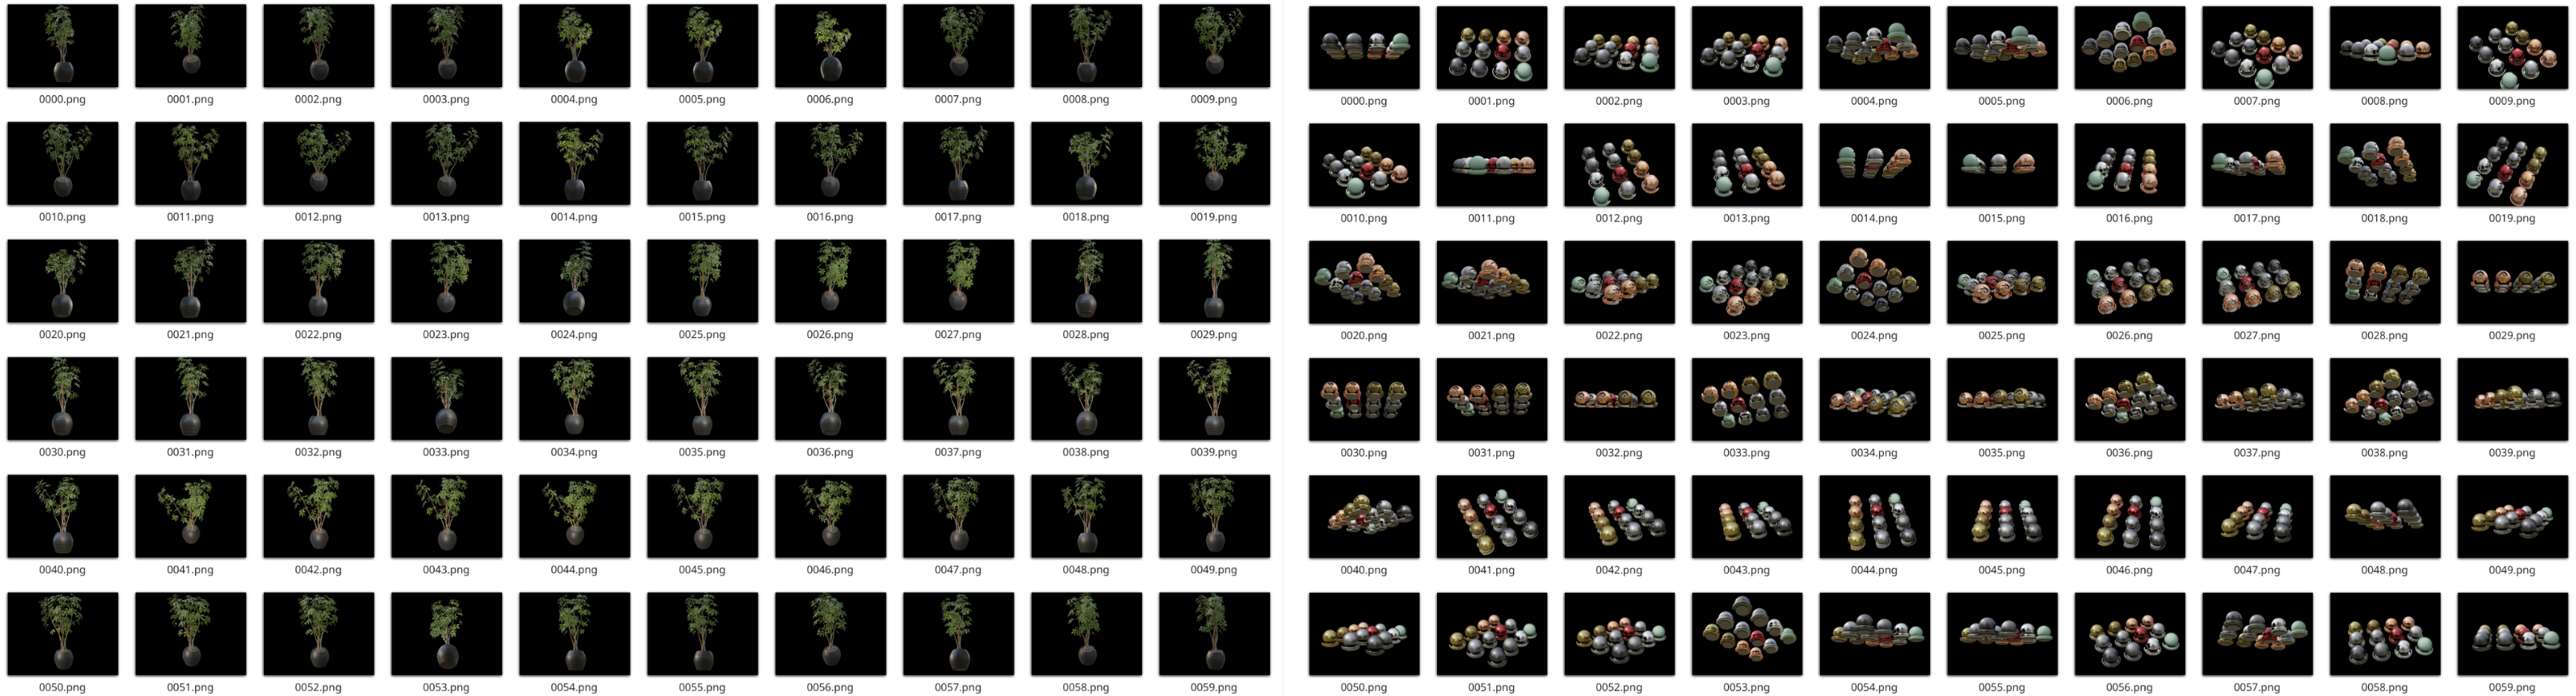
\includegraphics[width=0.5\textwidth]{figures/ficus_and_matballs.png}
    \caption{60 views of resolution 640x480 of the \texttt{Ficus} scene rendered in 12 minutes On the right, \texttt{material balls} scene rendered in a total of 25 minutes on a laptop equipped with a Nvidia T500.}
    \label{fig:multiview}
\end{figure}

The environment map does not appear as a backround (although it is possible in the current code) as it would allow to simplify and remove one of the extra components of the ADOP paper (e.g. it allows rendering the point cloud without using the neural environment map trick).

We parameterize camera orientation using 3 Euler Angles (yaw pitch roll) and 3 positions. We build the extrinsic camera matrix from the 3 angles and use a pinhole camera model to project 3D points onto the image plane as we'll see in ~\cref{sec:projecting_the_point_cloud_onto_the_image_plane}. There's a perfect equivalence between the camera parameters used in Blender and the ones used in my Pytorch renderer.

One of the difficulties of using synthetic rendering from meshes is that sometimes thin surfaces are modeled with double sided triangles. Since our rendering pipeline is using normal culling, we end up with an issue: points with normals not pointing towards the camera are not rendered. So on the ficus scene for instance, if we look "at the green leafs" from the bottom, the green leaves will become transparent so the renderer will have a hard time during reconstruction. We may therefore stick to objects with easy geometry such as the \texttt{old chair} scene. This is illustrated in \cref{fig:ficus_culling_issue}.

When working on natural scenes, the points will most probably be duplicated on both sides of the surface by COLMAP with the normals in both ways. In my case, I sampling points randomly from the mesh and I simply take the normal of the triangle to which the point belongs without considering it double sided.

I first notticed this effect on my synthetic \texttt{stair case} scene which was only made of planes and that could not be optimized in the trivial "Bypass" case.

\begin{figure*}
    \centering
    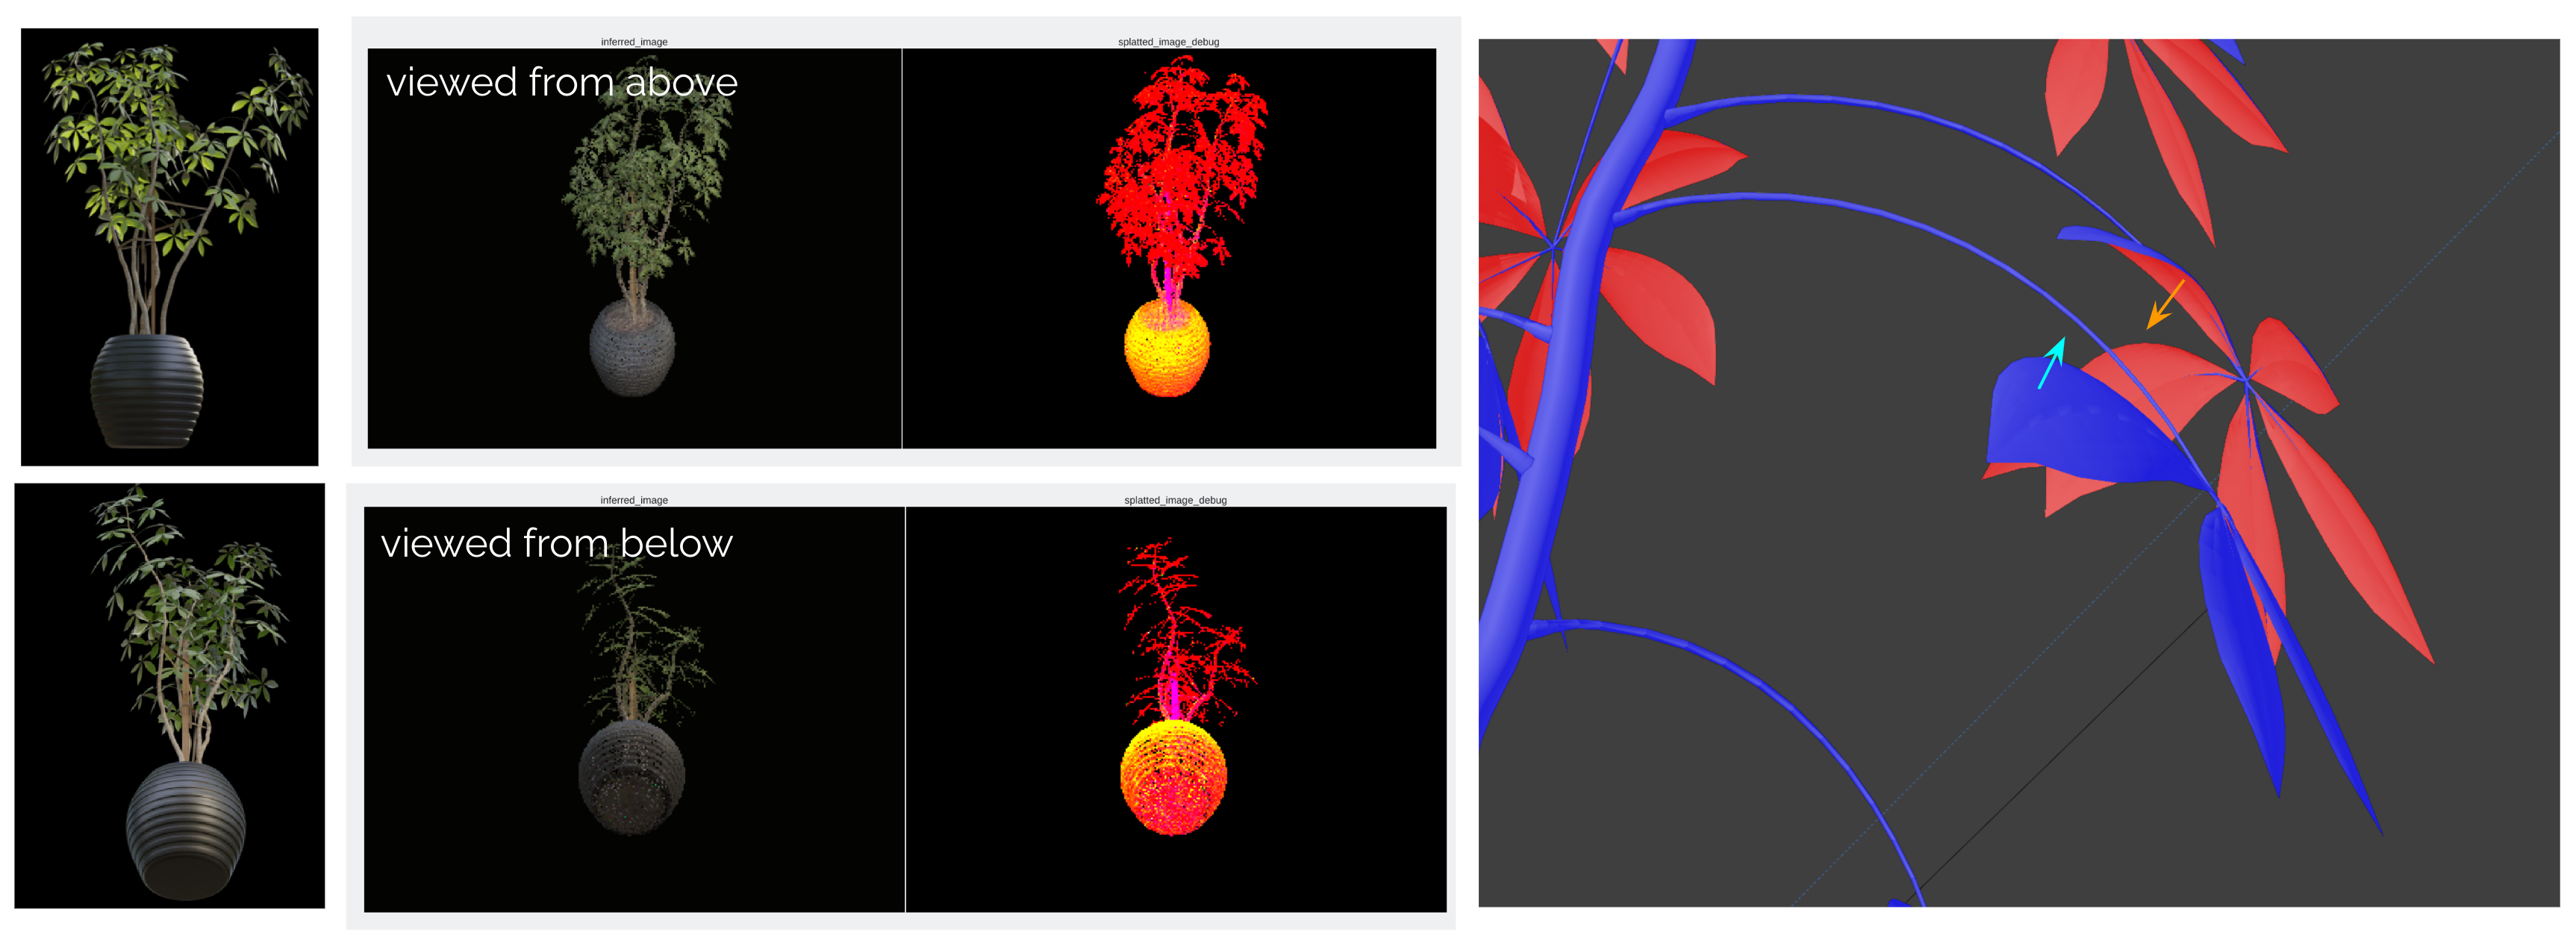
\includegraphics[width=0.8\textwidth]{figures/double_sided_surfaces_issues.png}
    \caption{On the left, image from the Blender render of the ficus scene, seen slightly from below where the leaves look brighter than when looked from above. On the right side, we check the rendering of the point cloud with the "Bypass" mode (which allows ajusting the colors points to the scene). Most leaves are oriented upwards so normal culling does not render these points when seen from below. The optimization process has trouble to reconstruct correct colors for the leaves. On the right side, the blender face orientation (blue front facing the camera/red back facing the camera) fully reveals that the leaves of the \texttt{ficus} scene are made of double sided triangles.}
    \label{fig:ficus_culling_issue}
\end{figure*}

\subsection{Projecting the point cloud onto the image plane}
\label{sec:projecting_the_point_cloud_onto_the_image_plane}

\subsubsection{Coordinates projection}
\label{sec:coordinates_projection}

\begin{figure}[H]
    \centering
    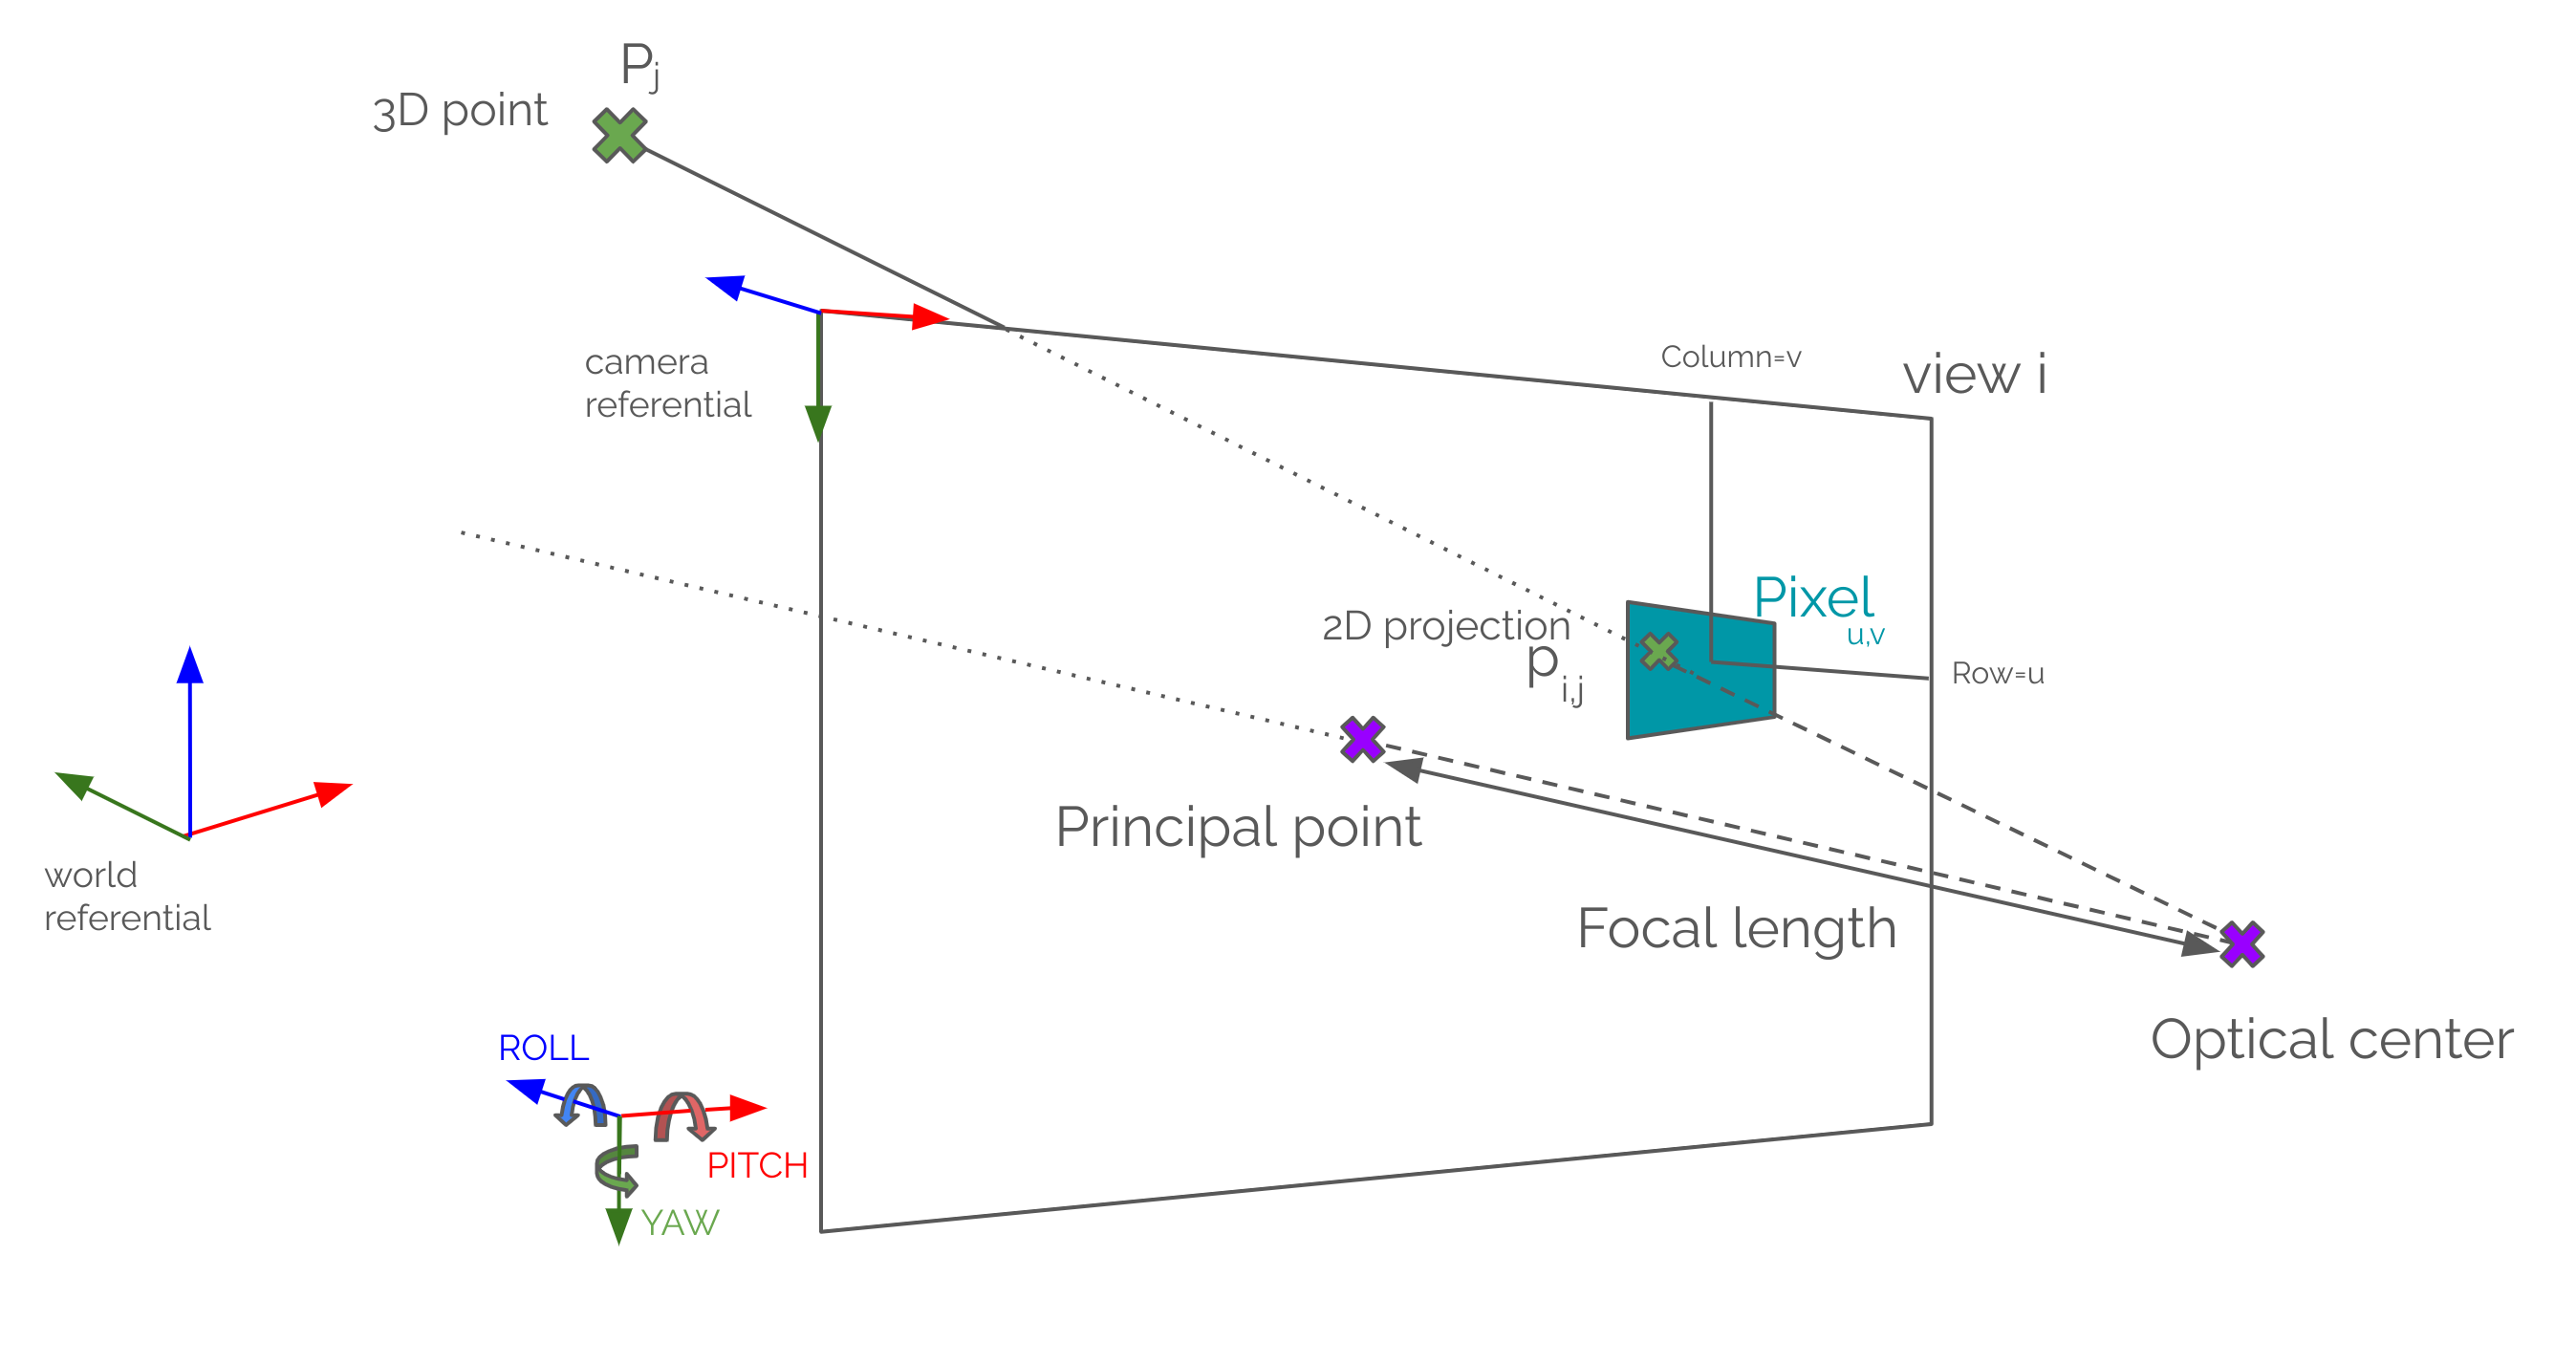
\includegraphics[width=0.4\textwidth]{figures/pinhole_camera_with_angles.png}
    \caption{Pinhole camera model. The $j^\text{th}$ point of the 3D point cloud, located at $\vec{P_{\textrm{3D}}}^{(j)}$ expressed in world coordinates is projected onto the sensor plane for view $i$ at position $\vec{p_{\textrm{2D}}}^{(i,j)}$ expressed as pixel coordinates, rounded to the 2D nearest integer coordinates $(u,v)$}
    \label{fig:pinhole_camera}
\end{figure}


To project a 3D point of index $j$ located at $\vec{P_{\textrm{3D}}}^{(j)}$ in world coordinates onto the image sensor,
we use the pinhole projection model as illustrated in \ref{fig:pinhole_camera}.

$$\vec{p_{\textrm{2D}}}^{(j)} = K\cdot\left[Q_{\text{cam}} | T_{\text{cam}}\right]^{i}\vec{P_{\textrm{3D}}}^{(j)}$$
where
\begin{itemize}
    \item $K$ is the camera 3x3 intrinsic matrix.
    \item $Q_{\textrm{cam}}^{i}$ is the camera orientation for view $i$, this matrix is created from the yaw, pitch, roll angles.
    \item $T_{\textrm{cam}}^{i}$ is the 3D camera position for view $i$ in the world frame (meters)
    \item $\vec{P_{\textrm{3D}}}^{(j)} \in \mathbb{R}^{4}$ are the homogeneous 3D coordinates of point $j$ in the world frame.
    \item $\vec{p_{\textrm{2D}}}^{(i,j)} \in \mathbb{R}^{3}$ are the homogeneous 2D coordinates of point $j$ projected in the sensor frame $i$ (pixel coordinates).
\end{itemize}

This operation is performed in ~\href{https://github.com/balthazarneveu/per-pixel-point-rendering/blob/main/src/pixr/rendering/forward_project.py}{\texttt{forward\_project.py}} in parallel over all points $j$ , using \texttt{torch.matmul} operation

\noindent \textit{Points coordinates could probably be projected all at once for all camera views using \texttt{torch.bmm}.}

\subsubsection{Scatter operation.}
\label{sec:scatter_op}

Visible points's colors are copied into corresponding pixels on the 2D image. A point only leads to a single pixel color update by taking the nearest pixel coordinate of $\lceil\vec{p_{\textrm{2D}}}^{(j)}\rfloor$. There are conditions to satisfy for each point to be valid. 
\begin{itemize}
    \item $(C1)$ The point must be inside the image frame $0\leq x<W$ and $0\leq y <H$.
    \item $(C2)$ The point must be in front of the camera ($Z>0$).
    \item $(C3)$ The normal of the point must be facing the camera.
    \item $(C4)$ The point must not be occluded by another point.
\end{itemize}

\noindent \textbf{Soft depth test.} 
That last condition requires some work:
Using a Z-buffer, it is possible to take the closest point to the camera. Since several points may fall into the same pixel cell, there will be aliasing as several pixels may be located on the same suface. The authors rely on previous work \cite{schutz2021rendering} to average pixels in a tiny range of depths behind the closest point. This is called a soft depth test and we'll describe this part in details as it required a tricky implementation with Pytorch.

\begin{figure}[H]
    \centering
    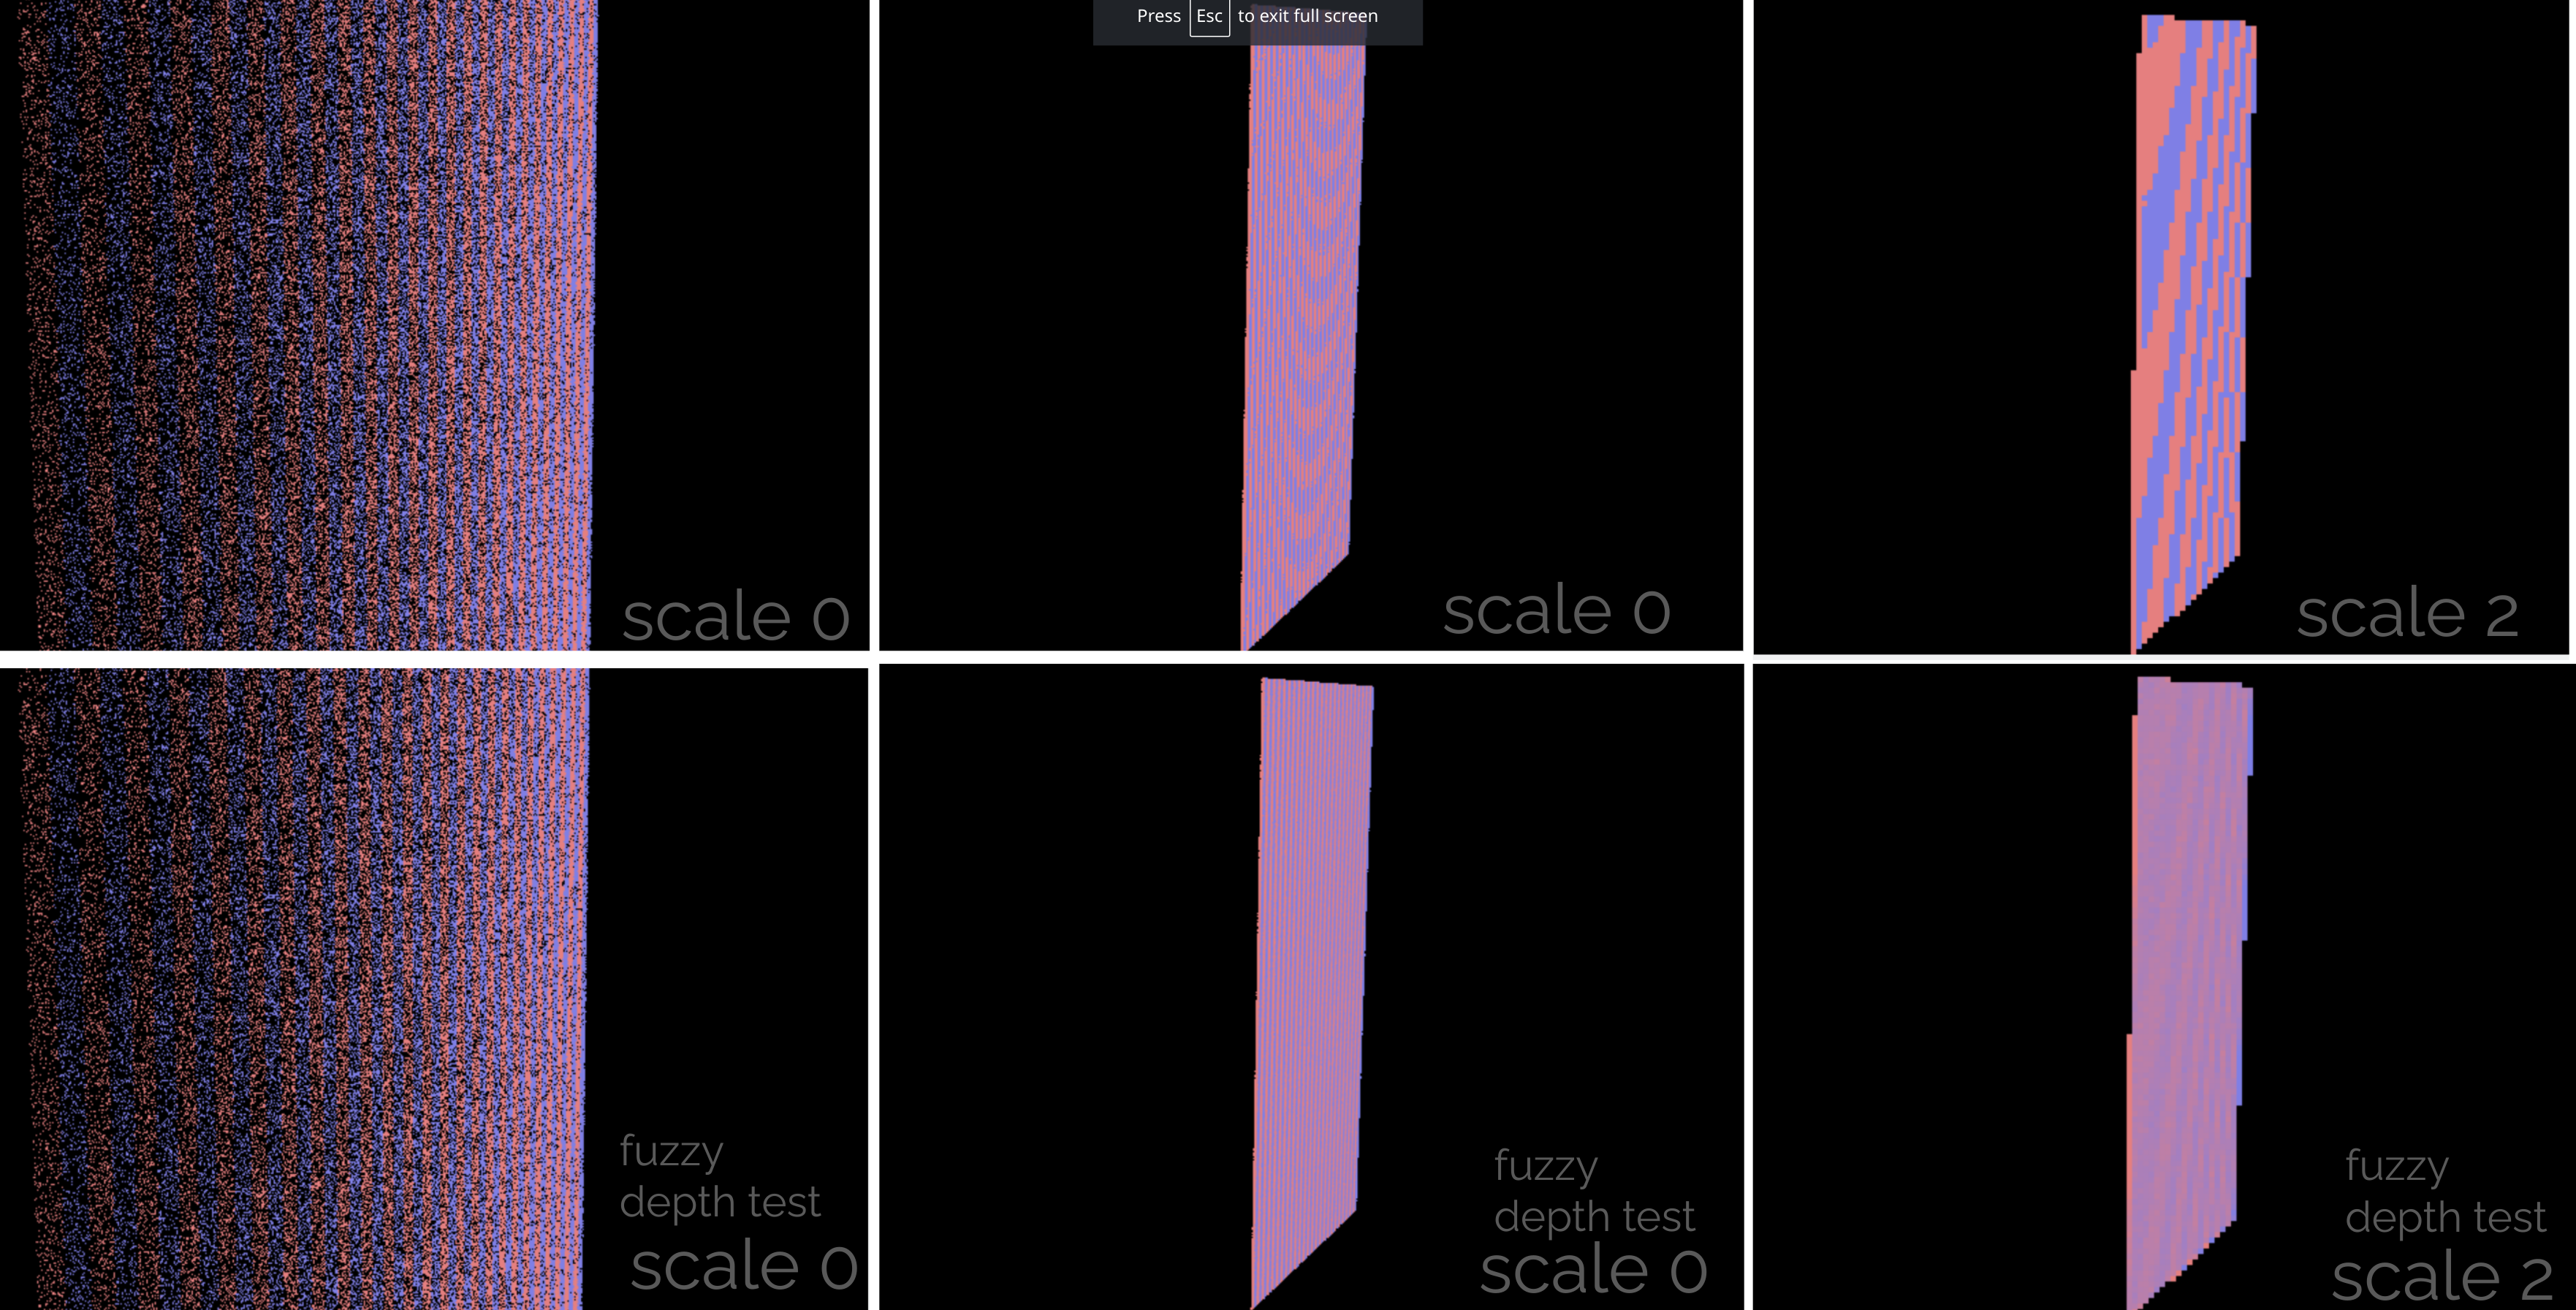
\includegraphics[width=0.5\textwidth]{figures/fuzzy_depth_test_aliasing_large.png}
    \caption{Fuzzy depth test acts as an anti-aliasing filter. On this test scene, a point cloud made of 500.000 point located in the same plane with an alternate vertical red an blue stripes on . We use $\alpha=0$ on the top (hard depth test) and $\alpha=0.01$ on the bottom (soft depth test). On the right side, when using larger scales (lower resolutions), aliasing effect if naturally amplified.}
    \label{fig:fuzzy_depth_test_AA}
\end{figure}

Soft depth test $Z \leq (1 + \alpha) * \textrm{min}_{Z_{j}}$ requires two passes. First compute the closest point to the camera for each pixel. Then, for each pixel, average the colors of the points that are close enough to the closest point. As we'll perform the first pass, we'll keep track of conditions $(C1)$, $(C2)$ and $(C3)$ to avoid recomputing them during the second pass.

\noindent \textbf{First pass: Hard depth test.}

\noindent ~\href{https://github.com/balthazarneveu/per-pixel-point-rendering/blob/main/src/pixr/rendering/zbuffer\_pass.py#L5}{\texttt{zbuffer\_pass.py}} is the first pass. It allows to find the closest point to the camera for each pixel. Depth values are initialized at $\inf$ and will remain $\inf$ when a pixel has not been filled. A first implementation trick is for each point of index $j$ to keep a linear index $k$ of its coordinate position in the image $k[j] = 1+ u*W+v$ if the point is valid regarding conditions $(C1)$, $(C2)$ and $(C3)$ and set this index to $k[j]=0$ otherwise. This allows to avoid recomputing the same test conditions during the second pass.

We then obtain the closest depth image for each pixel. $\forall (u,v) \in \left[0, H-1\right] \times \left[0, W-1\right]$:
$$Z^{\texttt{min}}_{(u,v)} = min_{\left\{j  \text{ s.t. } k[j]=1+u*W+v\right\}} \left(Z[j]\right)$$
\noindent Although this index mapping looks unnatural, it allows to use the ~\href{https://pytorch.org/docs/stable/generated/torch.Tensor.scatter\_reduce\_.html#torch.Tensor.scatter\_reduce\_}{\texttt{torch.scatter\_reduce\_}} operation to take the minimum of depth values for each pixel in a 1D tensor of size $1+W*H$.

My first ~\href{https://github.com/balthazarneveu/per-pixel-point-rendering/blob/main/src/pixr/rendering/legacy\_splatting.py}{\texttt{legacy\_splatting.py} implementation with a for loop} was way too slow and using native torch operators allowed me to get fast point cloud rendering (and save some development time to avoid rewriting a custom CUDA kernel).

\noindent \textbf{Second pass. Soft depth test and color aggregation}

In the second pass  ~\href{https://github.com/balthazarneveu/per-pixel-point-rendering/blob/main/src/pixr/rendering/colors\_aggregation.py}{rendering/colors\_aggregation.py}, we are now capable to apply the soft depth test as we have already computed the closest distance of the point cloud to the camera for each pixel. We'll modify the point index mapping $k[i]$ to only keep indices which satisfy the soft depth test: 
$$ k'[j] = k[j] * \left(Z[j] \leq (1+\alpha) *Z^{\texttt{min}}_{(u,v) \equiv k[j]}\right)$$.
Multiplying by the boolean tensor gracefully sets to 0 the indices which do not satisfy the condition and keeps the others unchanged. Keep in mind that the $k=0$ index is the invalid pixel and will be discarded.
Finally, we average the colors of the points that satisfy the soft depth test, at each pixel location, using \texttt{torch.scatter\_reduce\_} operator with the \texttt{reduce=`mean`}. It is possible to keep a background

\begin{figure*}[h]
    \centering
    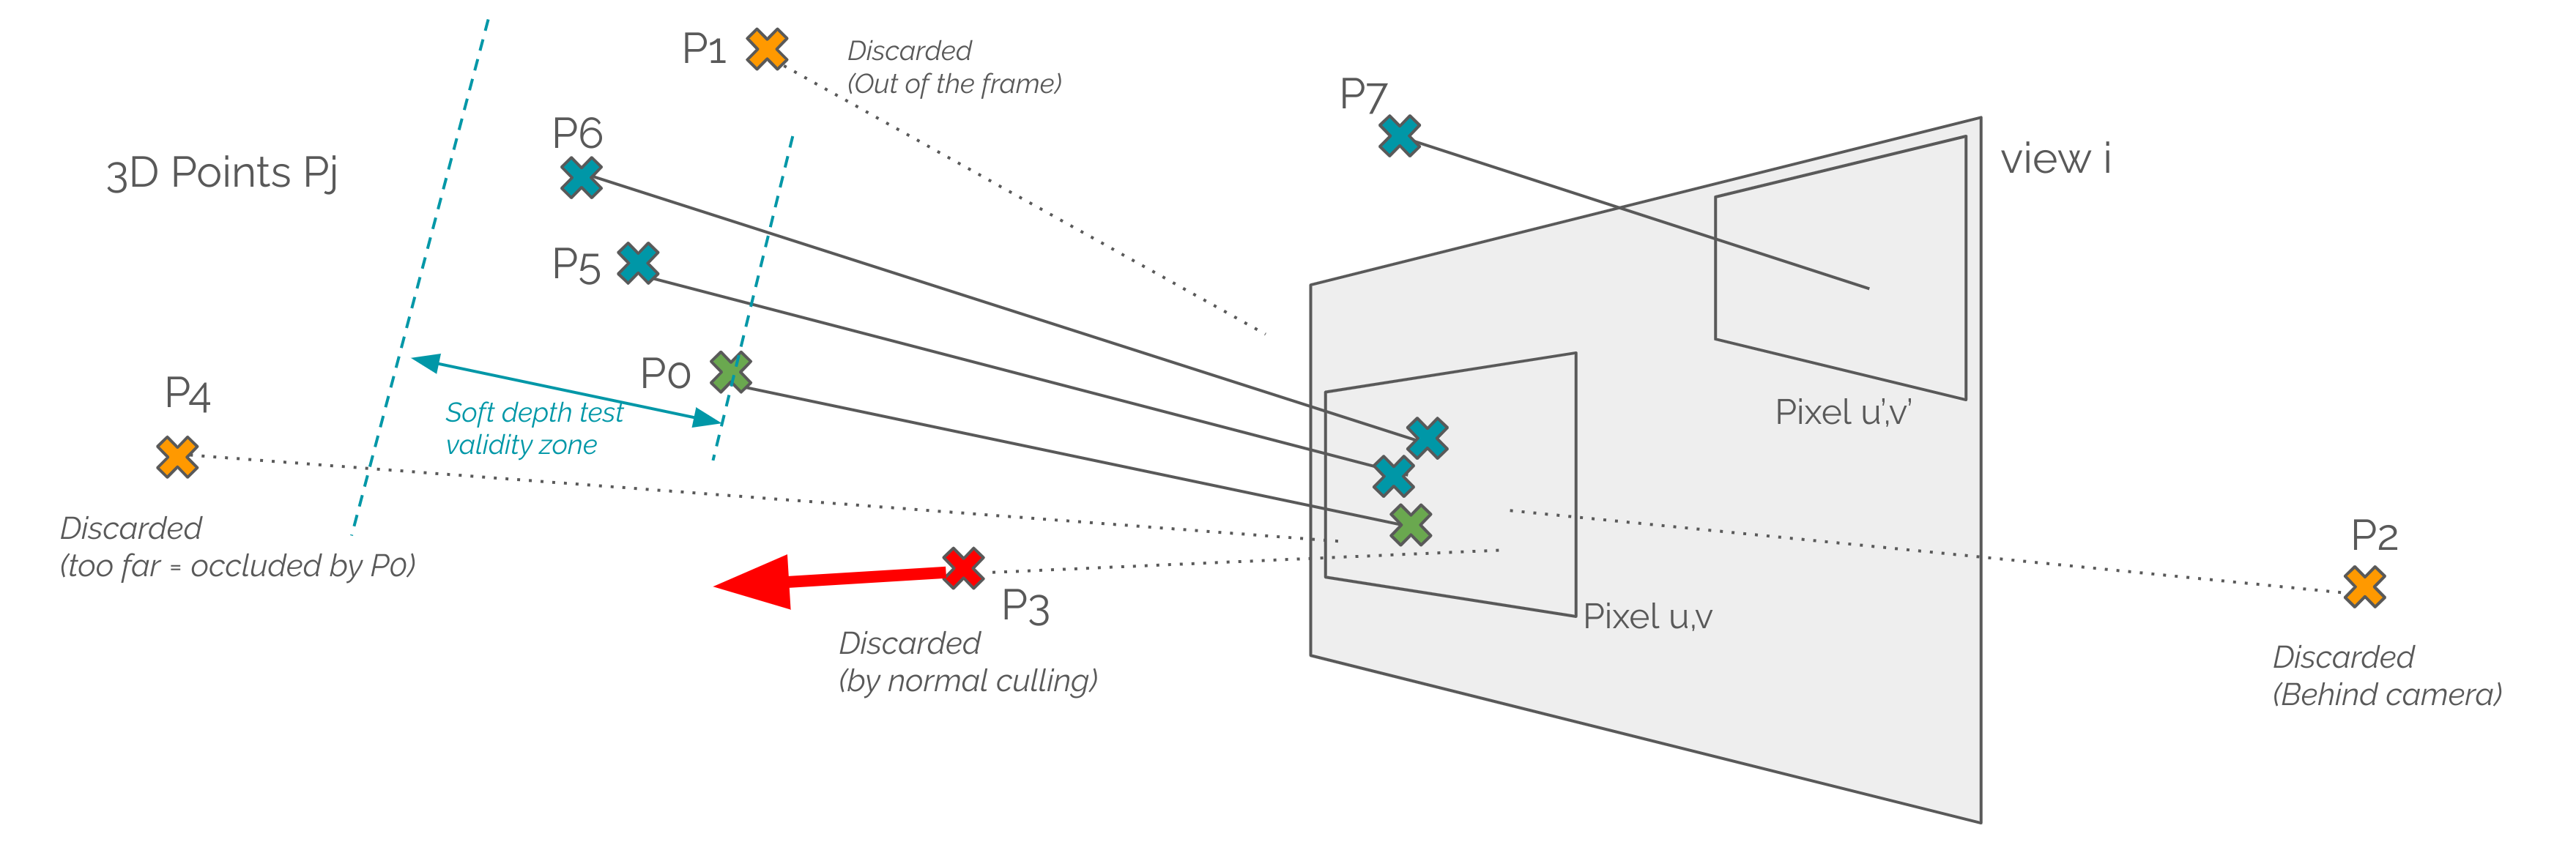
\includegraphics[width=0.9\textwidth]{figures/soft_depth_test_two_pixels.png}
    \caption{Soft depth test illustration: 
    $P^{(0)}$ is the closest point to the camera for pixel $(u,v)$. We will average the colors of the points $(P^{(0)}, P^{(5)}, P^{(6)})$. During the first pass, we'll keep track of the mapping between point indices and projected coordinates (in a 1D fashion). $k[0]=k[4]=k[5]=k[6]=1+u*W+v$ and $k[1]=k[2]=k[3]=0$, $k[7] = 1+u'*W+v'$. First pass will find the minimum of depths for each pixel $Z^{\texttt{min}}_{(u,v)} = min_{\left\{j  \text{ s.t. } k[j]=1+u*W+v\right\}} \left(Z[j]\right), \forall (u,v) \in \left[0, H-1\right] \times \left[0, W-1\right]$. For instance $Z^{\texttt{min}}_{(u,v)} = Z^{(0)}$ and $Z^{\texttt{min}}_{(u',v')} = Z^{(7)}$. \\ During the second pass, we'll only keep indices which satisfy the soft depth test: $ k'[j] = k[j] * \left(Z[j] \leq (1+\alpha) *Z^{\texttt{min}}_{(u,v) \equiv k[j]}\right)$.
   For instance, point 4 is considered too far away and discared e.g. $k[4]=0$. \\Finally, colors are averaged $I_{u, v} \propto \sum_{j \texttt{ s.t  } k'[j]=1+u.W+v}{I(j)}$. For instance $I_{(u, v)} = \frac{I(0) + I(5) + I(6)}{3}$ and $I_{(u', v')} = I(7)$.}
    \label{fig:soft_depth_test}
\end{figure*}
